\documentclass[12pt]{article}

\usepackage{blindtext} % Package to generate dummy text throughout this template 

\usepackage[utf8]{inputenc}
\usepackage{amsmath, amssymb}
\usepackage{algorithm}
\usepackage[noend]{algpseudocode}
\linespread{1.5}
\usepackage[margin = 1in]{geometry}
\usepackage{microtype} % Slightly tweak font spacing for aesthetics
\usepackage[english]{babel} % Language hyphenation and typographical rules
\usepackage{tikz}
\usepackage{pgfplots}
%\tikzexternalize
\usepackage{hyperref}
\usepackage{url}
\usepackage{graphicx}
\usepackage{float}
\usepackage{wrapfig}
\usepackage{multicol}
\usepackage{subcaption}
\usepackage{nomencl}
\usepackage[titletoc, page]{appendix}
\usepackage{caption}
\captionsetup{font={small}}
\hypersetup{
    colorlinks=true,
    linkcolor=black,      
    urlcolor=red,
    bookmarks=true,
    citecolor=green!75!black
}

\setlength{\parindent}{2em}
%\setlength{\parskip}{1.5em}
\graphicspath{ {images/} }

% nomenclature specs
\makenomenclature
\renewcommand{\nomname}{List of Commonly Used Functions, Symbols \& Terms}
%% This code creates the groups
% -----------------------------------------
\usepackage{etoolbox}
\renewcommand{\nomgroup}[1]{%
    \item[\bfseries
    \ifstrequal{#1}{T}{Terms}{%
        \ifstrequal{#1}{S}{Symbols}{%
            \ifstrequal{#1}{F}{Functions}{}}%
    }]}
% -----------------------------------------

\newcommand{\vect}[1]{\mathbf{#1}}  % vector
\newcommand{\matr}[1]{\mathbf{#1}}  % matrix
\newcommand{\tens}[1]{\mathbf{#1}}  % tensor
\newcommand{\mean}[1]{\overline{#1}}    % mean overline

\begin{document}
    % nomenclature
    \mbox{}
    % symbols
    \nomenclature[S]{$\matr{M}$; $\matr{m}$}{Matrix or vector depending on the context}
    \nomenclature[S]{$J$}{Number of locations in the dataset}
    \nomenclature[S]{$T$}{Number of time units for which data is available}
    
    % functions
    \nomenclature[F]{softmax($\cdot$)}{Defined as softmax($z_i$) = $\frac{\exp(z_i)}{\sum_{i} \exp(z_i)}$}
    \nomenclature[F]{reLU($\cdot$)}{Defined as reLU($z$) = max(0, $z$)}
    \nomenclature[F]{batch-multiply($\cdot$)}{Operates on $m \times n \times p$ and $m \times p \times q$ tensors to give a $m \times n \times q$ tensor.}
    \printnomenclature[1.5in]
    \cleardoublepage
    
    \tableofcontents
    \listoftables
    \listoffigures
    
    % main body
    \section{Introduction} \label{sec:Introduction}
    Optimizing predictive models on datasets that are obtained from citizen-science projects can be computationally expensive as these datasets grow in size with time. Consequently, models based on multiple-layered neural networks, Integer Programming and other optimization routines can prove increasingly difficult as the number of parameters increase, despite using the faster Central Processing Units (CPUs) in the market. Incidentally, it becomes difficult for citizen-science projects to scale if the organizers use CPUs to run optimization models. However, Graphical Processing Units (GPUs), which offer multiple cores to parallelize computation, can outperform CPUs in computing such predictive models if these models heavily rely on large-scale matrix multiplications. By using GPUs over CPUs to accelerate computation on a citizen-science project, the model could achieve better optimization in less time, enabling the project to scale.\\
    
    Part of the eBird project, which aims to ``maximize the utility and accessibility of the vast numbers of bird observations made each year by recreational and professional bird watchers'', Avicaching is a incentive-driven game trying to homogenize the spatial distribution of citizens' (agents') observations [cite website]. Since the dataset of agents' observations in eBird is geographically heterogeneous (concentrated in some places like cities and sparse in others), Avicaching homogenizes the observation set by rewarding agents who visit under-sampled locations \cite{Xue2016Avi1}. To accomplish this task of specifying rewards at different locations based on the historical records of observations, Avicaching would learn the change in agents' behavior when a certain sample of rewards were applied to the set of locations, and then distribute a newer set of rewards across the locations based on those learned parameters \cite{Xue2016Avi2}. This requirement naturally translates into a predictive optimization problem, which is implemented using multiple-layered neural networks and linear programming.

    \subsection{Computation Using GPUs} \label{sec:comp_using_GPUs}
    
    \section{Problem Formulation} \label{sec:Problem Formulation}
    Since NVIDIA General Purpose GPUs enable faster computation on matrices, accelerated through CUDA and cuDNN, both the Identification (Section \ref{sec:Identification Problem}) and the Pricing Problem (Section \ref{sec:Pricing Problem}) were formulated as 3-layered and 2-layered neural networks respectively, using the PyTorch library.
    
    \subsection{Identification Problem} \label{sec:Identification Problem}
    As discussed in Section \ref{sec:Introduction}, the model should learn parameters that caused the change in agents' behavior when a certain set of rewards was applied to locations in the experiment region. Specifically, given datasets $\vect{y_t}$ and $\vect{x_t}$ of agents' visit densities with and without the rewards $\vect{r_t}$, we want to find weights $\matr{w_1}$ and $\matr{w_2}$ that caused the change from $\vect{x_t}$ to $\vect{y_t}$, factoring in possible influence from environmental factors $\matr{f}$ and distances between locations $\matr{D}$. Although the original model proposed to learn a single set of weights $\matr{w}$ \cite{Xue2016Avi2}, this proposed model considers two sets of weights $\matr{w_1}$ and $\matr{w_2}$ as it may theoretically result into higher accuracy and lower loss. Mathematically, the model can be formulated as:
    \begin{equation} \label{eq:iden_problem}
    \begin{aligned}
    & \underset{\matr{w_1}, \matr{w_2}}{\text{minimize}}
    & & Z_I(\matr{w_1}, \matr{w_2}) = \sum_{t} (\omega(\vect{y_t} - \matr{P}(\matr{f}, \vect{r_t}; \matr{w_1}, \matr{w_2})\vect{x_t}))^{2}
    \end{aligned}
    \end{equation}
    where $\omega$ is a set of weights at time $t$ capturing penalties relative to the importance of homogenizing at different locations and elements $p_{u, v}$ of $\matr{P}$ are given as:
    \begin{equation} \label{eq:puv_equation}
    p_{u, v} = \frac{\exp(\matr{w_2} \cdot \text{reLU} (\matr{w_1} \cdot [d_{u, v}, \vect{f_{u}}, r_{u}]))}{\sum_{u'} \exp(\matr{w_2} \cdot \text{reLU} (\matr{w_1} \cdot [d_{u', v}, \vect{f_{u'}}, r_{u'}]))} = \frac{\exp(\Gamma_{u, v})}{\sum_{u'}\exp(\Gamma_{u', v})} = \text{softmax}(\Gamma_{u, v})
    \end{equation}
    In the expression for $p_{u,v}$ (Equation \ref{eq:puv_equation}), softmax$(\cdot)$ is the function: softmax$(z_i) = \frac{\exp(z_i)}{\sum_{i}\exp(z_i)}$ and the reLU$(\cdot)$ function is a ``rectified Linear Unit'' defined as: reLU$(z) = \text{max}(0, z)$.\\
    To optimize the loss value $Z_I(\matr{w_1}, \matr{w_2})$ (Equation \ref{eq:iden_problem}), the neural network learns the set of weights through multiple epochs \nomenclature[T]{Epoch}{One training/testing period; iteration}of backpropagating the loss using gradient descent. Furthermore, the program processes the dataset before feeding to the network to avoid unnecessary sub-epochs and promote batch operations on matrices. 
    
    \subsubsection{Structure of Input Dataset for Identifying Weights} \label{sec:Structure of Input Dataset for Identifying Weights}
    \begin{figure}[H]
        \begin{subfigure}{.64\textwidth}
            \centering
            \includegraphics[width=\linewidth]{weights_input_dataset}
            \caption{A Tensor representing the Input Dataset $\matr{F}$}
            \label{fig:A Tensor representing the complete Input Dataset}
        \end{subfigure}
        \begin{subfigure}{.35\textwidth}
            \centering
            \includegraphics[width=\linewidth]{zoomup_Fuv}
            \caption{Contents of $\matr{F}[v][u]$}
            \label{fig:Zoomed-in contents of Fvu}
        \end{subfigure}
        \caption{Visual representation of the Input Dataset}
        \label{fig:Visual representation of the Input Dataset}
    \end{figure}
    Since preprocessing the dataset impacts the efficiency of the network, the input dataset, comprising of distance between locations $\matr{D}$, environmental features $\vect{f}$ and given rewards $\vect{r_t}$ (all normalized) are combined in a specific manner. Since GPUs are efficient in operating on matrices and tensors, the input dataset is built into a tensor (Figure \ref{fig:A Tensor representing the complete Input Dataset}) such that batch operations could be performed on slices $\matr{F}[v]$. Another advantage of building the dataset as a tensor comes with the PyTorch library, which provides convenient handling and transfer of tensors residing on CPUs and GPUs. Algorithm \ref{alg:Constructing the Input Dataset} describes the steps to construct this dataset.
    \begin{algorithm}
        \caption{Constructing the Input Dataset} \label{alg:Constructing the Input Dataset}
        \begin{algorithmic}[1]
            \Function{Build-Dataset}{$\matr{D}, \matr{f}, \matr{r_t}$}
            \State $\matr{D} \gets \Call{Normalize}{\matr{D}}$\Comment{$\matr{D}[u][v]$ is the distance between locations $u$ and $v$}
            \State $\vect{f} \gets \Call{Normalize}{\mathbf{f}, axis = 0}$\Comment{$\mathbf{f}[u]$ is a vector of env. features at location $u$}
            \State $\vect{r_t} \gets \Call{Normalize}{\vect{r_t}, axis = 0}$\Comment{$\vect{r_t}[u]$ is the reward at location $u$}
            \For{$v = 1, 2, \dots, J$}
                \For{$u = 1, 2, \dots, J$}
                    \State $\tens{F}[v][u] \gets [\matr{D}[v][u], \vect{f}[u], \vect{r_t}[u]]$ \Comment{As depicted in Figure \ref{fig:Zoomed-in contents of Fvu}}
                 \EndFor
            \EndFor
            \State \Return $\matr{F}$
            \EndFunction
        \end{algorithmic}
    \end{algorithm}
       
    \subsubsection{Minimizing Loss for the Identification Problem} \label{sec:Minimizing Loss for the Identification Problem}
    As shown in Figure \ref{fig:Neural network designed for the Identification Problem}, the neural network is made of 3 fully connected layers - the input layer, the hidden layer with rectified Linear Units (reLU), and the output layer generating the results using the softmax$(\cdot)$ function. The network can also be visualized as a collection of 1-dimensional layers (Figure \ref{fig:Side view of the network}), with the softmax$(\cdot)$ calculated on the collection's output.
    \begin{figure}[H]
        \begin{subfigure}{.64\textwidth}
        \includegraphics[width=\textwidth]{weights_net}
        \caption{3-dimensional view of the network slice, taking in $\matr{F}[v]$}
        \label{fig:3-dimensional view of the network slice, taking in Fv}
        \end{subfigure}
        \begin{subfigure}{.35\textwidth}
            \includegraphics[width=\textwidth]{weights_net_side}
            \caption{Side view of the network}
            \label{fig:Side view of the network}
        \end{subfigure}
        \caption{Neural network designed for the Identification Problem}
        \label{fig:Neural network designed for the Identification Problem}
    \end{figure}
    It is important to clarify that the network in Figure \ref{fig:3-dimensional view of the network slice, taking in Fv}, which takes in $\matr{F}[v]$ as shown, is a slice of the original network, which takes in the complete tensor $\matr{F}$ and computes the complete result $\matr{P}^{T}$  per iteration of $t$. In other words, the input and the hidden layers are 3-dimensional, and the output layer is 2-dimensional. Since it is difficult to visualize the complete network on paper, slices of the network are depicted in Figure \ref{fig:3-dimensional view of the network slice, taking in Fv}. Algorithm \ref{alg:Algorithm for the Identification Problem per epoch} details the steps for learning the parameters $\matr{w_1}$ and $\matr{w_2}$ based on Equations \ref{eq:iden_problem} \& \ref{eq:puv_equation}.\\
    \begin{algorithm}
        \caption{Algorithm for the Identification Problem per epoch} \label{alg:Algorithm for the Identification Problem per epoch}
        \begin{algorithmic}[1]
            \Require $\matr{w_1}, \matr{w_2}, T$
            \Function{Identify-Weights}{$\matr{x}, \matr{y}, \matr{r}, \matr{D}, \matr{f}, \omega$}
            \For{$t = 1, 2, \dots, T$}
                \State $\matr{F} \gets \Call{Build-Dataset}{\matr{D}, \matr{f}, \matr{r}[t]}$\Comment{Defined in Algorithm \ref{alg:Constructing the Input Dataset}}
                \State $\matr{\Lambda} \gets \text{reLU}(\Call{Batch-Multiply}{\matr{F}, \matr{w_1}})$\Comment{\textbf{Phase 1: Feed Forward}}
                \State $\matr{\Gamma} \gets \text{softmax}(\Call{Batch-Multiply}{\matr{\Lambda}, \matr{w_2}})$
                \State $\matr{P} \gets \matr{\Gamma}^T$
                \State $loss \gets loss + (\omega(\matr{y}[t] - \matr{P} \cdot \matr{x}[t]))^2$
            \EndFor
            \State $\Call{Gradient-Descent}{loss, \matr{w_1}, \matr{w_2}}$\Comment{\textbf{Phase 2: Backpropagate}}
            \State $\matr{w_1}, \matr{w_2} \gets \Call{Update-Using-Gradients}{\matr{w_1}, \matr{w_2}}$
            \State \Return $loss$
            \EndFunction
        \end{algorithmic}
    \end{algorithm}
    
    \subsection{Pricing Problem} \label{sec:Pricing Problem}
    After learning the set of weights $\matr{w_1}$ and $\matr{w_2}$ highlighting the change in agents' behavior to collect observations, the Pricing Problem aims to redistribute rewards to the all locations such that the predicted behavior of agents influenced by the new set of rewards is homogeneous. Thus, given a budget of rewards $\mathcal{R}$, this optimization problem can be expressed as:
    \begin{equation} \label{eq:pricing_problem}
    \begin{aligned}
    & \underset{\vect{r}}{\text{minimize}}
    & & Z_P(\vect{r}) = \frac{1}{n}\lVert \vect{y} - \mean{\vect{y}} \rVert\\
    & \text{subject to}
    & & \vect{y} = \matr{P}(\matr{f}, \vect{r}; \matr{w_1}, \matr{w_2}) \, \vect{x}\\
    &&& \sum_{i} r_i \leq \mathcal{R}\\
    &&& r_i \geq 0
    \end{aligned}
    \end{equation}
    where elements of $\matr{P}$ are defined as in Equation \ref{eq:puv_equation}. 
    To allocate the rewards $\vect{r}$ optimally, the calculations for the pricing problem are akin to that for the Identification Problem (Section \ref{sec:Identification Problem}). However, since only 1 set of rewards need to be optimized, we use an altered 2-layer network instead of the 3-layer network used to identify the weights. While Equation \ref{eq:pricing_problem} looks like a typical Linear Programming problem, only a part of the formulation uses Linear Programming to constrain the rewards. The more computationally expensive part (calculation for $\matr{P}$ on a CPU) is modeled as a 2-layer network that minimizes the loss function $Z_P(\vect{r})$ using gradient descent. Although this use of a neural network may seem similar to that of the Identification Problem, there are major changes in the structure of the network used here. These alterations for the Pricing Problem and differences from the Identification Problem are discussed further in the following sections.
    
    \subsubsection{Input Dataset for Finding Rewards}
    
    Since it is the set of rewards $\vect{r}$ that need to be optimized, they must serve as the ``weights'' of the network (note that ``weights'' refer to the edges of this network and not to the set of calculated weights $\matr{w_1}$ and $\matr{w_2}$). Therefore, the rewards $\vect{r}$ are no longer fed into the network but are its characteristic. Instead, the calculated weights $\matr{w_1}$ are fed into the network, and are ``weighted'' by the rewards.\\
    
    The observation density datasets, $\matr{x}$ and $\matr{y}$, are also aggregated for all agents such that they give information in terms of locations $u$ only. This is also why rewards $\vect{r}$ does not depend on $t$ - we want a generalized set of rewards for all time $t$ per location $u$. Therefore, the algorithm for constructing $\matr{F}$ (Section \ref{sec:Structure of Input Dataset for Identifying Weights}) is same as Algorithm \ref{alg:Constructing the Input Dataset} but with a change - $\vect{r_t}$ replaced by $\vect{r}$.
    
    \subsubsection{Optimizing \& Constraining Rewards} \label{sec:Optimizing and Constraining Rewards}
    The algorithm for finding $\matr{P}$ is very similar to Phase 1 of Algorithm \ref{alg:Algorithm for the Identification Problem per epoch} but without any epochs of $t$, as $\vect{x}$ is a vector rather than a matrix. Also, since the program would predict $\vect{y}$, it does not need labels $\vect{y}$ as a dataset.\\
    
    \begin{algorithm}
        \caption{Solving the Pricing Problem} \label{alg:Solving the Pricing Problem}
        \begin{algorithmic}[1]
            \Function{Optimize-Rewards}{$\vect{x}, \matr{w_1}, \matr{w_2}, \matr{D}, \matr{f}$}
            \Require $\vect{r}, \mathcal{R}$
            \State $\matr{F} \gets \Call{Build-Dataset}{\matr{D}, \matr{f}, \vect{r}}$\Comment{Defined in Algorithm \ref{alg:Constructing the Input Dataset}}
            \State $\matr{\Lambda} \gets \text{reLU}(\Call{Batch-Multiply}{\matr{F}, \matr{w_1}})$\Comment{\textbf{Phase 1: Solve for $\matr{P}$ and $loss$}}
            \State $\matr{\Gamma} \gets \text{softmax}(\Call{Batch-Multiply}{\matr{\Lambda}, \matr{w_2}})$
            \State $\matr{P} \gets \matr{\Gamma}^T$
            \State $\vect{y} \gets \matr{P} \cdot \vect{x}$
            \State $loss \gets \lVert \vect{y} - \mean{\vect{y}} \rVert / J$\Comment{$J$ is the number of locations}
            \State $\Call{Gradient-Descent}{loss, \vect{r}}$\Comment{\textbf{Phase 2: Backpropagate}}
            \State $\vect{r} \gets \Call{Update-Using-Gradients}{\vect{r}}$
            \State $\vect{r} \gets \Call{LP}{\vect{r}, \mathcal{R}}$\Comment{LP($\cdot$) explained below}
            \State \Return $loss$
            \EndFunction
        \end{algorithmic}
    \end{algorithm}
    After updating the rewards, the program constrains them using LP($\cdot$) such that $\sum_{i}r_i \leq \mathcal{R}$ and $r_i \geq 0$. To do so, the LP($\cdot$) finds another set of rewards $\vect{r'}$ such that the absolute difference between new and old rewards ($\sum_{i}|r'_i - r_i|$) is minimum. The mathematical formulation is given in Equation \ref{eq:lp_math_constrain_rewards}, which was implemented using SciPy's Optimize Module []. Since the module supports a standard format\footnote{minimize [$\vect{c}^T \cdot \vect{x}$]; subject to [$\matr{A} \cdot \vect{x} \leq \vect{b}, \, x_i \geq 0$] \label{foot:lp standard format}} for doing linear programming, Equation \ref{eq:lp_code_constrain_rewards} (after rearranging constraints and building $\matr{A}, \vect{b}$ and $\vect{c}$) is used, which is mathematically equivalent to Equation \ref{eq:lp_math_constrain_rewards}.
    \begin{multicols}{2}
        \begin{equation} \label{eq:lp_math_constrain_rewards}
        \begin{aligned}
            & \underset{\vect{r'}}{\text{minimize}}
            & & \sum_{i}|r'_i - r_i|\\ \\
            & \text{subject to}
            & & \sum_{i}r'_i \leq \mathcal{R}\\
            &&& r_i \geq 0
        \end{aligned}
        \end{equation}\break
        \begin{equation} \label{eq:lp_code_constrain_rewards}
        \begin{aligned}
            & \underset{\vect{r'}, \vect{u}}{\text{minimize}}
            & & \sum_{i} u_i\\
            & \text{subject to}
            & & r'_i - r_i \leq u_i\\
            &&& r_i - r'_i \leq u_i\\
            &&& \sum_{i} r'_i \leq \mathcal{R}\\
            &&& r'_i, u_i \geq 0
        \end{aligned}
        \end{equation}
    \end{multicols}

    \section{Experiment Specifications} \label{sec:Experiment Specifications}
    To test both our models, we conducted several tests for optimization and GPU speedup over CPU. After initializing all parameters randomly and reading data from files, the models were run for 1000 to 10000 epochs depending on the complexity of the model and any potential benefits emerging with more epochs. \\
    
    A Dell Precision Tower 3620 with Intel Core i7-7700K Processor, 16GB RAM and NVIDIA Quadro P4000 GPU with 1792 CUDA Cores was used for all experiments, which were run on original datasets for optimization tests and randomly generated datasets for GPU speedup tests. We believe that speedup tests on original datasets would give similar results, though we used randomly generated datasets because it was easier to scale the sizes of random data and test on a variety of dataset sizes.\\
    
    Note that operations in the scripts were distributed between CPU and GPU when GPU is mentioned as ``set'', while the operations were executed only on the CPU when the ``CPU'' is mentioned as set. Since GPUs are inferior than CPUs at handling most operations other than simple arithmetic matrix ones, we used - and recommend using - both the CPU and the GPU in the former case (GPU ``set'') to handle operations they are superior at. However, since the models in Sections \ref{sec:Identification Problem} and \ref{sec:Pricing Problem} (not the full scripts) are primarily arithmetic operations on matrices and tensors, it is clear that they were executed on the GPU when it was ``set'' and on the CPU when the CPU was ``set''.
    
    On the algorithm side, we used Adam's algorithm for \textsc{Gradient-Descent}($\cdot$), after testing performances of several algorithms including but not limited to Stochastic Gradient Descent (SGD) [], Adam's Algorithm [] and RMSProp [] (PyTorch lets you choose the corresponding function). Since Adam's algorithm was found to work best with both models over all test runs, all experiments were done using Adam's algorithm.
    
    \subsection{Running the Identification Problem's Model}
    \subsubsection{Optimizing the Original Dataset}
    The 3-layered neural network was run for 10000 epochs on the original dataset, which was split 80:20 for training and testing sets, with learning rate = 0.01. Since we were aiming for optimization, we ran multiple tests (5 different seeds) of the model only with the GPU ``set''.\\
    
    To compare this model's optimization results with other model structures, the previously studied 2-layered network \cite{Xue2016Avi2} and a 4-layered neural network were used. The 4-layered network had another hidden layer with reLU, equivalent to the hidden layer in the current 3-layered network (Figure \ref{fig:3-dimensional view of the network slice, taking in Fv}). The results from the 2-layered network were obtained from the study, and those from the 4-layered network were attained on the same original dataset with same parameter values (learning rate, epochs etc.).
    
    \subsubsection{Testing GPU Speedup on the Random Dataset}
    After generating random datasets of different sizes ($T = 17, 85, 173$ - Section \ref{sec:Minimizing Loss for the Identification Problem}, we ran our 3-layered model on each dataset size with different seeds with both GPU and CPU ``set''.
    
    \subsection{Running the Pricing Problem's Model}
    \subsubsection{Optimizing the Original Dataset}
    After obtaining the set of weights $\matr{w_1}$ and $\matr{w_2}$ optimized using different seeds, we tested to find the best rewards (with the lowest loss - Equation \ref{eq:pricing_problem}) with random $\vect{r}$ initiation. To average the results, the model was run several times on the same set of weights, using different set of weights (obtained from running the Identification Problem with different seeds) each time. Specifically, we ran the Pricing Problem's model 5 times (each with different seeds) for each set of weights, which were itself 5 in number.
    
    \subsubsection{Testing GPU Speedup on the Random Dataset}
    After generating random datasets of different sizes ($J = 11, 55, 116$ - Section \ref{sec:Minimizing Loss for the Identification Problem}), we ran our 3-layered model on each dataset size with different seeds with both GPU and CPU ``set''.
    
    \section{Results} \label{sec:Results}
    \subsection{Identification Problem's Results}
    Minimizing the loss function in the Identification Problem (Section \ref{sec:Identification Problem}) on the original dataset for 10000 epochs took an average of 1260.62 seconds with the GPU ``set''.
    \begin{itemize}
        \item The average loss values at the end of 10000 epochs were 0.04 on the training set and 0.14 on the test set.
        \item The average loss values for the 4-layered model (for comparison) with same experiment specifications were 0.14 on the training set and 0.49 on the test set.
    \end{itemize}
    \begin{wrapfigure}{r}{.5\textwidth}
        \centering
        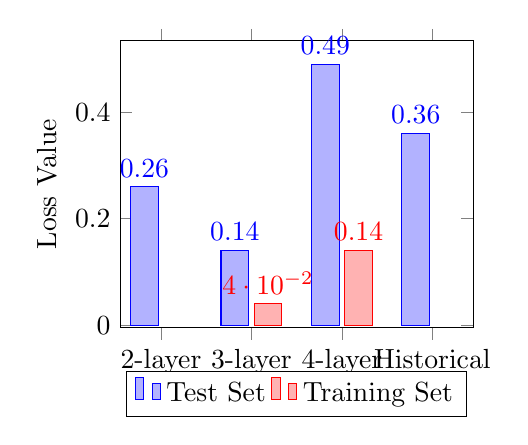
\begin{tikzpicture}
        \begin{axis}[
        ybar,
        width=.5\textwidth,
        enlarge x limits=0.15,
        legend style={at={(0.5,-0.15)},
            anchor=north,legend columns=-1},
        ylabel={Loss Value},
        symbolic x coords={2-layer,3-layer,4-layer, Historical},
        xtick=data,
        nodes near coords,
        nodes near coords align={vertical},
        ]
        \addplot coordinates {(2-layer,0.26) (3-layer,0.14) (4-layer,0.49) (Historical, 0.36)};
        \addplot coordinates {(3-layer,0.04) (4-layer,0.14)};
        \legend{Test Set,Training Set}
        \end{axis}
        \end{tikzpicture}
        \caption{Comparison of Loss Values from different models of the Identification Problem}
        \label{fig:Comparison of Loss Values from different models of the Identification Problem}
    \end{wrapfigure}

    As depicted in Figure \ref{fig:Comparison of Loss Values from different models of the Identification Problem}, our 3-layered neural network outperformed the previous 2-layered model by 0.12 units (12\% more closer to Ground Truth \cite[Table 1]{Xue2016Avi2}), and also produced much better results (35\% more closer to Ground Truth) than the 4-layered model. \\
    
    Although there remained a 10\% difference (0.10 loss units) in the values of training and testing set, the 3-layered model was not starkly overfitting as the $10\pm2\%$ difference persisted for the many epochs, instead of increasing and tuning more to the training set. This result is shown in Figure \ref{fig:Train & Test Loss Values' Plots of Different Models} with plots of loss values at each epoch for the 3- and the 4-layered network.
    \begin{figure}[h]
        \centering
        \begin{subfigure}{.49\textwidth}
            \centering
            \includegraphics[width=\textwidth]{weights_train_test_loss_plot}
            \caption{Plot for 3-layered Model}
            \label{fig:Plot for 3-layered Model}
        \end{subfigure}
        \begin{subfigure}{.49\textwidth}
            \centering
            \includegraphics[width=\textwidth]{weights_train_test_loss_plot}
            \caption{Plot for 4-layered Model}
            \label{fig:Plot for 4-layered Model}
        \end{subfigure}
        \caption{Train \& Test Loss Values' Plots for One of the Runs of Different Models}
        \label{fig:Train & Test Loss Values' Plots of Different Models}
    \end{figure}
    
    \subsection{Pricing Problem's Results}
    \section{Conclusion} \label{sec:Conclusion}
    
    \blindtext
    \bibliographystyle{ieeetr}
    \bibliography{avicaching}
    
    \cleardoublepage
    \begin{appendices}
    \section{Implementation} \label{sec:Implementation}
    The code can be found here[]. \\
    Both the Identification and the Pricing Problem were programmed in Python 2.7 using NumPy 1.12.1, SciPy 0.19.1 and PyTorch 0.1.12 modules [web cites] \cite{SCPOptimizeDocs}\cite{NPDocs}. [Results from Python plotted in Matplotlib 2.0.2] With some code optimizations, the input dataset $\matr{F}$ was built using NumPy's \texttt{ndarray} and PyTorch's \texttt{tensor} functions. Since PyTorch offers NumPy-like code base but with dedicated neural network functions and submodules, PyTorch's \texttt{relu} and \texttt{softmax} functions were used along with other matrix operations.\\
    
    \subsection{Specific Implementation Details for the Pricing Problem}
    Among all the code optimizations in both models, some in that for the Pricing Problem are worth discussing, as they drastically differ from Algorithm \ref{alg:Solving the Pricing Problem} or are intricate. Most optimizations relevant to the Identification Problem are trivial and relate directly to those for the Pricing Problem. Therefore, only those in the Pricing Problem model are discussed.
    
    \subsubsection{Building the Dataset $\matr{F}$}
    Notice that we build the dataset $\matr{F}$ and batch-multiply it with $\matr{w_1}$ on each iteration/epoch (lines 2-3 of Algorithm \ref{alg:Solving the Pricing Problem}). Doing these steps are repetitive as most elements of $\matr{F}$, distances $\matr{D}$ and environmental feature vector $\vect{f}$, do not change unlike rewards $\vect{r}$. Moreover since $\matr{w_1}$ is fixed, Algorithm \ref{alg:Solving the Pricing Problem} would repetitively multiply the $\vect{f}$ and $\matr{D}$ components of $\matr{F}$ with $\matr{w_1}$. To avoid these unnecessary computations, we preprocessed most of $\matr{F}$ by batch-multiplying with $\matr{w_1}$ and only multiplied $\vect{r}$ with the corresponding elements of $\matr{w_1}$. Figure \ref{fig:Splitting and Batch Multiplying F and w1} describes the process graphically.\\
    \begin{figure}[!htbp]
        \centering
        \includegraphics[width=\linewidth]{split_and_batch_multiply}
        \caption{Splitting and Batch Multiplying $\matr{F}$ and $\matr{w_1}$}
        \label{fig:Splitting and Batch Multiplying F and w1}
    \end{figure}    
    Although this preprocessing might seem applicable for the model in Identification Problem too, it does not apply fully. Since the weights $\matr{w_1}$ are updated on each iteration/epoch, we cannot multiply them with parts of $\matr{F}$ beforehand (Algorithm \ref{alg:Algorithm for the Identification Problem}). However, we can combine $\matr{D}$ and $\vect{f}$ in the preprocessing stage and simply append $\vect{r}[t]$ on each iteration, saving computation time.
    
    \subsubsection{Modeling the Linear Programming Problem in the Standard Format}
    The \texttt{scipy.optimize} module's \texttt{linprog} function requires that the arguments are in standard LP format. As discussed in \cref{sec:Calculating Rewards}, Equation \ref{eq:lp_code_constrain_rewards} resembles the standard format more closely than \ref{eq:lp_math_constrain_rewards}, but it may not be clear how so.\\
    
    Considering $\vect{u}$ and $\vect{r'}$ as variables $\vect{x}$, Equation \ref{eq:lp_code_constrain_rewards} translates into Equation \ref{eq:lp_matrix_rewards} ($J$ is the number of locations).
    \begin{equation} \label{eq:lp_matrix_rewards}
    \begin{aligned}
    & \text{minimize}
    & & \begin{bmatrix}
    \vect{0_J}\\
    \vect{1_J}\\
    \end{bmatrix}^T
    \begin{bmatrix}
    \vect{r'}\\
    \vect{u}
    \end{bmatrix}\\ \\
    & \text{subject to}
    & & \begin{bmatrix}
    I_J & -I_J\\
    -I_J & -I_J\\
    \vect{1}^T_J & \vect{0}^T_J\\
    \end{bmatrix}
    \begin{bmatrix}
    \vect{r'}\\
    \vect{u}\\
    \end{bmatrix} \leq
    \begin{bmatrix}
    \vect{r}\\
    -\vect{r}\\
    \mathcal{R}\\
    \end{bmatrix}\\
    &&& r'_i, u_i \geq 0
    \end{aligned}
    \end{equation}
    
    \section{Strange GPU Speedup in LP Computation} \label{sec:Strange GPU Speedup in LP Computation}
    Even though we intentionally transferred the rewards vector to and constrained it using \texttt{scipy.optimize} module's \texttt{linprog} function on the CPU, we obtained an unexpected GPU speedup in the runtimes (see \cref{sec:PriProbRes - GPU} and Figure \ref{fig:Finding Rewards - Time taken by the LP}). Confounded by this weird behavior, we wanted to pinpoint the reasons because SciPy's function could not have differentiated between the configurations and delivered different results. However, since this was not our research's prime motive, we did not take a strong quantitative approach in determining the cause(s). There could have been many reasons for this bizarre behavior, including but not limited to:
    \begin{enumerate}
        \item SciPy's Optimize Module differentiating between configurations. This can be ruled out because the module could not have known the configuration during which it was called. This is because the configuration settings were applicable only on user-programmed operations, and needed to be explicitly stated - as mandated by PyTorch \cite{PTDocs}. SciPy's Optimize Module identifying the configurations is just supernatural.
        \item CPU ``set'' using exploiting more main memory than GPU ``set''. We suspected that since CPU ``set'' configuration's operations were executed solely on the CPU, the residing datasets could have used more main memory than when GPU ``set'' was running. This could have hampered the performance of LP with CPU ``set''. Unlike the 1\textsuperscript{st} possibility, this would have meant that CPU ``set'' was slowing down the LP, and not that GPU ``set'' was speeding up the LP.
    \end{enumerate}

    The 2\textsuperscript{nd} hypothesis/possibility seemed more promising than the others, and we built some programs to test its various aspects, which are elaborated in next sections.
    
    \subsection{Main Memory Usage by Both Configurations}
    As the initial approach, we logged details of main memory usage when the models were running. Contrary to our expectations (again), the GPU ``set'' was utilizing more main memory than CPU ``set'' was. Precisely, when running the Pricing Problem's model with $T = 173, J = 116$ without GUI and logging at 0.2 second intervals until the model completed, the GPU ``set'' was using 9.0 - 9.1 \% of the main memory, whereas CPU ``set'' was using only 0.9 \% memory. During the tests, only 1 CPU core was utilized for GPU ``set'', whereas 6-8 cores were being used for CPU ``set''. Clearly, main memory usage wouldn't have been the reason for the strange GPU speedup in LP runtime as LP's GPU ``set'' runtime would have been lower if the relation with main memory usage was true. However, there could be a relation between CPU usage and LP runtime.
    
    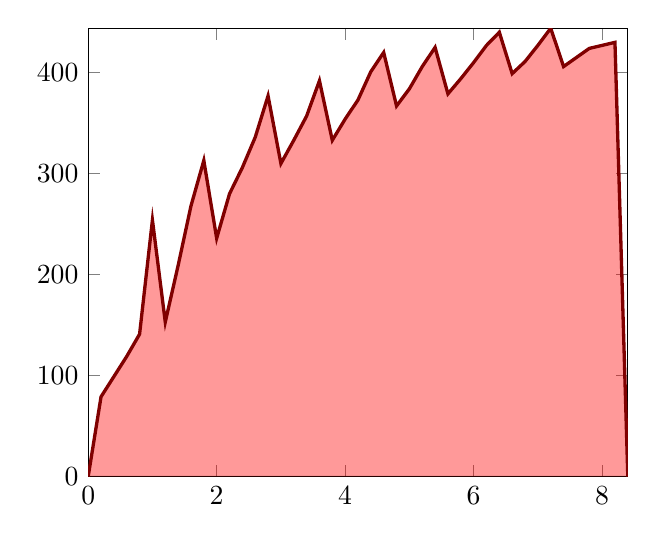
\begin{tikzpicture}
    \begin{axis}[
    domain=0:10,
    enlargelimits=false,
    ]
    %
    \addplot[fill=red, opacity=.4, domain=0:10] coordinates {
        (0.0, 0)
        (0.2, 79.0)
        (0.4, 99.0)
        (0.6, 119)
        (0.8, 141)
        (1.0, 254)
        (1.2, 153)
        (1.4, 209)
        (1.6, 268)
        (1.8, 313)
        (2.0, 236)
        (2.2, 280)
        (2.4, 306)
        (2.6, 336)
        (2.8, 377)
        (3.0, 310)
        (3.2, 333)
        (3.4, 357)
        (3.6, 392)
        (3.8, 333)
        (4.0, 354)
        (4.2, 373)
        (4.4, 401)
        (4.6, 420)
        (4.8, 367)
        (5.0, 384)
        (5.2, 406)
        (5.4, 425)
        (5.6, 379)
        (5.8, 394)
        (6.0, 410)
        (6.2, 427)
        (6.4, 440)
        (6.6, 399)
        (6.8, 411)
        (7.0, 427)
        (7.2, 444)
        (7.4, 406)
        (7.6, 415)
        (7.8, 424)
        (8.0, 427)
        (8.2, 430)
        (8.4, 0)
    }\closedcycle;
    
    \addplot [very thick, red!50!black] coordinates {
        (0.0, 0)
        (0.2, 79.0)
        (0.4, 99.0)
        (0.6, 119)
        (0.8, 141)
        (1.0, 254)
        (1.2, 153)
        (1.4, 209)
        (1.6, 268)
        (1.8, 313)
        (2.0, 236)
        (2.2, 280)
        (2.4, 306)
        (2.6, 336)
        (2.8, 377)
        (3.0, 310)
        (3.2, 333)
        (3.4, 357)
        (3.6, 392)
        (3.8, 333)
        (4.0, 354)
        (4.2, 373)
        (4.4, 401)
        (4.6, 420)
        (4.8, 367)
        (5.0, 384)
        (5.2, 406)
        (5.4, 425)
        (5.6, 379)
        (5.8, 394)
        (6.0, 410)
        (6.2, 427)
        (6.4, 440)
        (6.6, 399)
        (6.8, 411)
        (7.0, 427)
        (7.2, 444)
        (7.4, 406)
        (7.6, 415)
        (7.8, 424)
        (8.0, 427)
        (8.2, 430)
        (8.4, 0)
    };
    \end{axis}
    \end{tikzpicture}
    
    \subsubsection{asdf}
\end{appendices}
\end{document}